\pagebreak
\section{Implementation}
This section describes Java code and Eclipse specific implementation details
of the plug in. The plug in is composed of 5 Eclipse projects, 4 generated from
the Ecore model and 1 from the Sirius specification. See figure \ref{fig:projects}
for the list of projects.

\begin{figure}[h]
    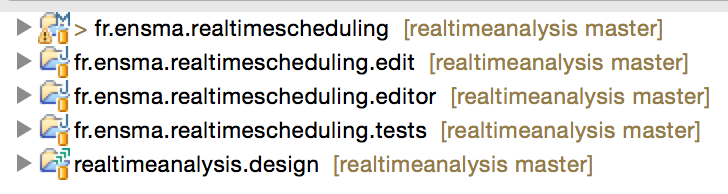
\includegraphics[width=0.5\textwidth]{eclipse_projects}
    \caption{Plug in projects}
    \label{fig:projects}
\end{figure}

Most of the non-generated code resides in \texttt{fr.ensma.realtimescheduling}, specifically
the analysis algorithms, visualization classes, and the meta-model interfaces and
implementations. This project will be refered to as the \textbf{main} project.

The projects \texttt{edit}, \texttt{editor}, and \texttt{test} contain
\textit{generated} code for editing the model
(operations such as instance creation, or attribute modification),
the editor GUI (see figure \ref{fig:model_editor}), and test code respectively. The test
project is currently not used.

Several Eclipse extensions are also declared in the \texttt{plugin.xml}
within the main project (see figure \ref{fig:eclipse_extensions}). These
mainly consist of UI extensions to allow for easier manipulation and analysis
of a model.
\subsection{Main Project}
The main project contains the analysis algorithms and non-trivial UI logic code for the 
project. The package structure of this project is given in figure \ref{fig:packages}.
\begin{figure}[h]
    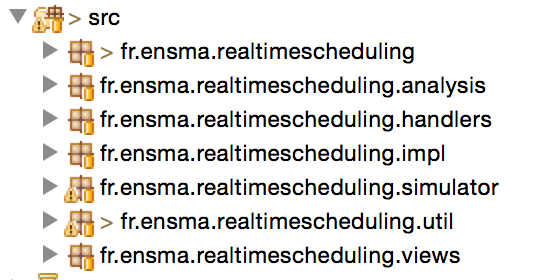
\includegraphics[width=0.4\textwidth]{packages}
    \caption{Main project packages}
    \label{fig:packages}
\end{figure}
Several of these packages deserve special attention.
\begin{description}
    \item[analysis] This package contains the algorithms and ``glue'' code between the model and the
    algorithms. The \texttt{Analyzer.java} class holds the implementations of all the algorithms
    described in the CORAC-PANDA project: the response time analysis from chapter 2 and the
    network delay analysis from chapter 3. The code was written attempting to recreate as much
    as possible the structure and names of the pseudo-code from the report. 
    \\
    The \texttt{ModelInterface.java} class contains methods to interface between the UI and the
    analysis algorithms.
    \\
    The rest of the classes in the package provide side-effect free functions for manipulating
    the model or classes to store auxilary data necessary by the algorithms.
    For example, the Ecore list implementation \texttt{EList} is not modifiable
    thus it cannot be passed to Java Collections methods such as \texttt{Collections.sort()}.
    Having a list of time-sorted \texttt{Interval}s is necessary for the algorithms thus
    the \texttt{PartitionUtils.java} file provides such a method by creating a copy of the original
    list.
    \item[handlers] This package contains handler definitions for the commands generated by
    Eclipse. UI actions in Eclipse are handled by a command-handler relationship. More information
    on this mechanic can be found online.
    \item[views] This package contains the classes used to layout and display data to charts from 
    the model. This project uses the \href{http://www.jfree.org/jfreechart/}{\textbf{JFreeChart}}
    library to generate charts like line charts and bar charts. The classes \texttt{AbstractLineChart.java} 
    and \texttt{AbstractBarChart.java} set up the layout of the charts which is a horizontal layout
    with a chart on the left and a control component on the right. 
    % TikZ diagram here
    \item[util] This package is generated by Ecore, however it houses the \texttt{RealtimeschedulingValidator.java}     class which contains the complex validation code that could not be expressed in OCLinEcore. The specifics
    of the validation are in section \ref{metamodel}.
\end{description}
\subsection{Edit}
This project contains generated code for modifying elements of a model instance. The only
modifications to this code are found in the \texttt{getText()} method of some of the instances
which makes the display in the editor more user friendly. See figure \ref{fig:model_editor}.
\subsection{Editor}
This project defines the generated classes for a simple model editor which
only displays a tree representation of the model.
\begin{figure}[h]
    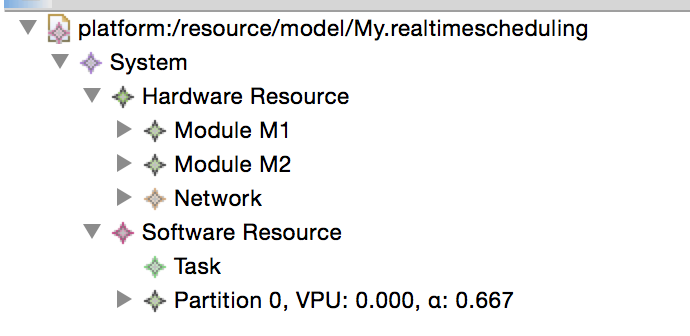
\includegraphics[width=0.4\textwidth]{model_editor}
    \caption{Model editor in use}
    \label{fig:model_editor}
\end{figure}
\subsection{Sirius Editor}
A view definition project was also created with the intent of making the network
definition easier. Editors that this project provides are only available in the 
runtime instance of Eclipse
\subsection{Eclipse Extensions}
The plug in provides several custom Eclipse extensions apart from the generated ones.
\begin{figure}[h]
    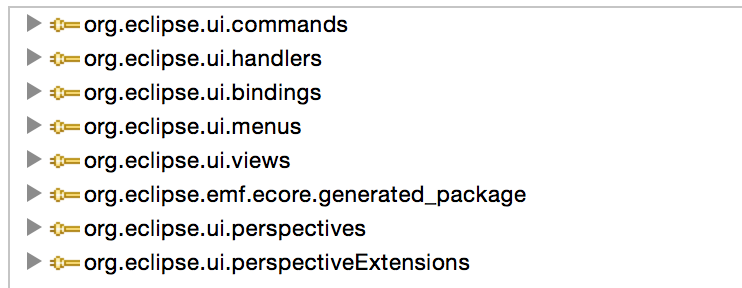
\includegraphics{eclipse_extensions}
    \caption{Plug in extensions}
    \label{fig:eclipse_extensions}
\end{figure}
\begin{description}
    \item[Menu] Menu extensions add items to existing menus. In this case, I added a menu item
    to the main Eclipse menu bar (see figure \ref{fig:menu_extension}). This is indicated by the root \textbf{Menu Contribution} element
    of the extension which indicates that this menu should be added to the menu specified by
    \texttt{menu:org.eclipse.ui.main.menu}.
    \begin{figure}[h]
        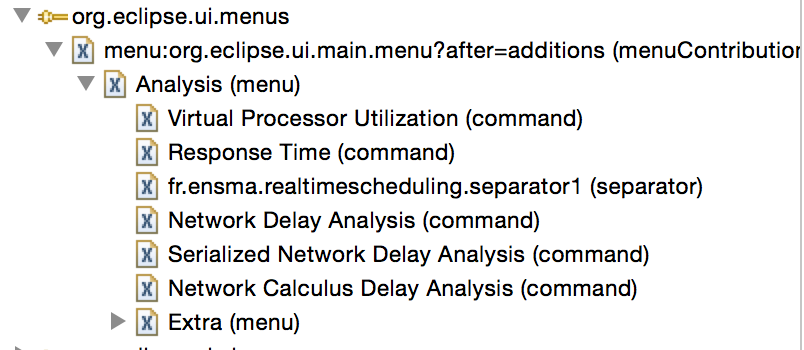
\includegraphics[width=0.4\textwidth]{menu_extension}
        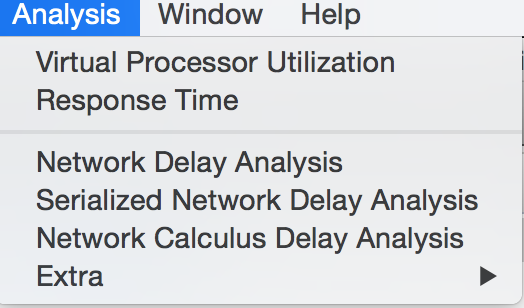
\includegraphics[width=0.3\textwidth]{menu_action}
        \caption{Menu extension definition and result}
        \label{fig:menu_extension}
    \end{figure}
    \item[View] Several new views are defined in the project. These are mainly for graphing
    the information derived from the analysis of the model.
    \begin{figure}[h]
        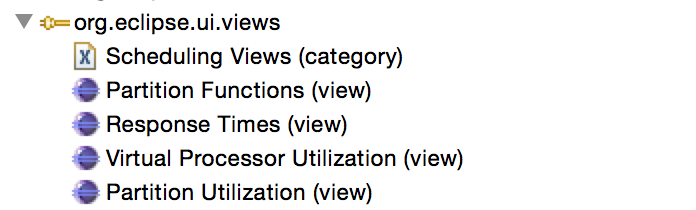
\includegraphics[width=0.45\textwidth]{view_extension}
        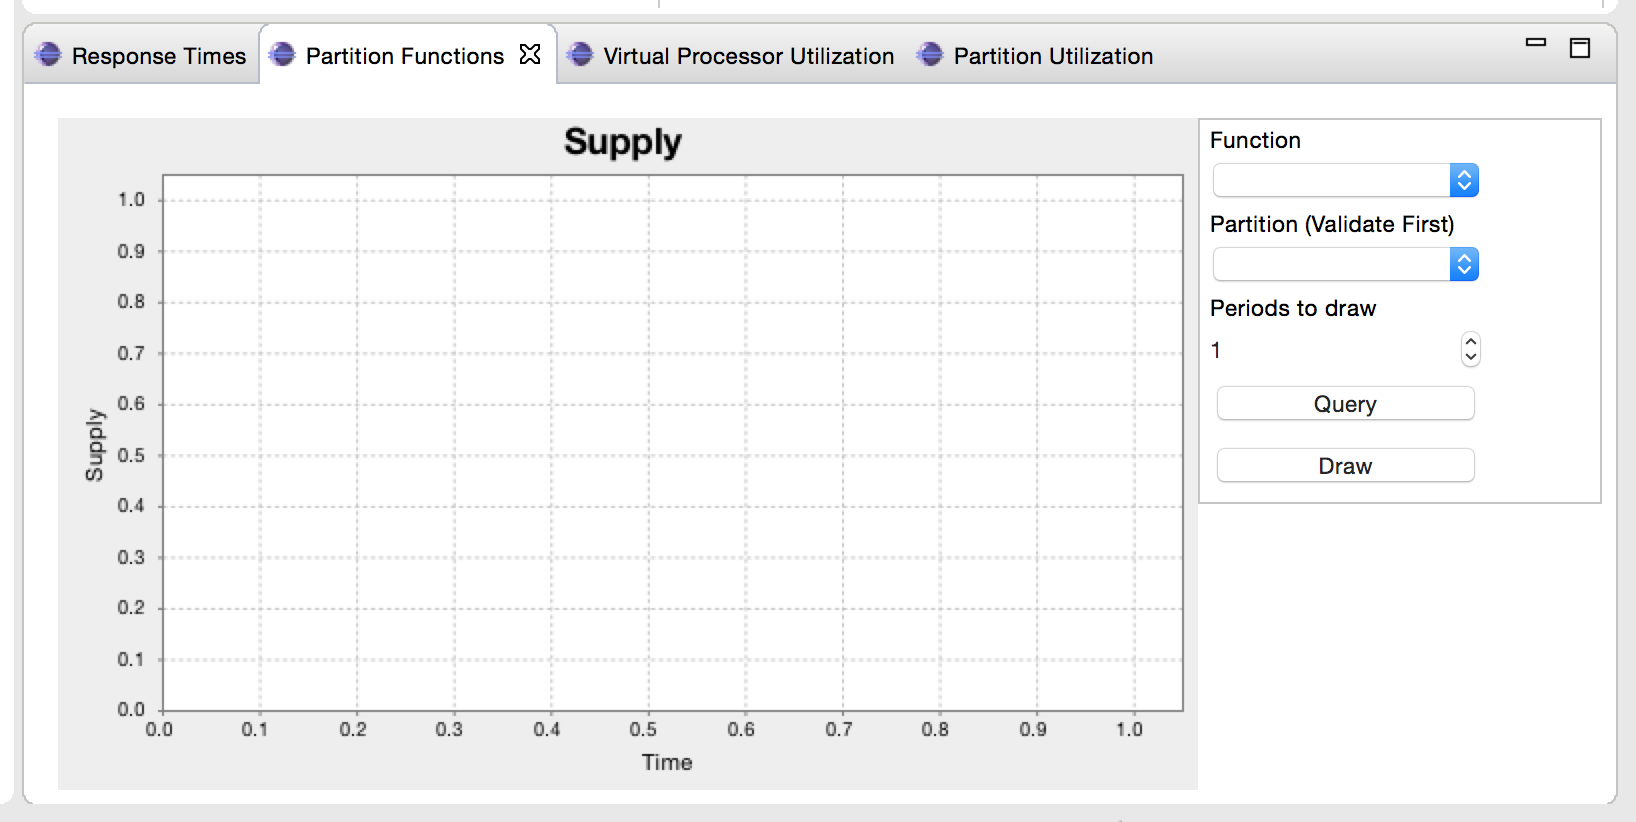
\includegraphics[width=0.45\textwidth]{view_action}
        \caption{View extension defition and result}
        \label{view_extension}
    \end{figure}
    \item[Perspective] One new perspective is declared with the purpose of arranging the model editor and the 
    graphing views into a coherent layout. New perspectives can be defined by first creating an extension of
    \texttt{org.eclipse.ui.perspective} and then of \texttt{org.eclipse.ui.perspectiveExtensions}. The
    first is a manifest to Eclipse that this plug-in defines a new extension; the second allows you
    to define the layout of the extension from within the \texttt{plugin.xml} editor. 
    \begin{figure}[h]
	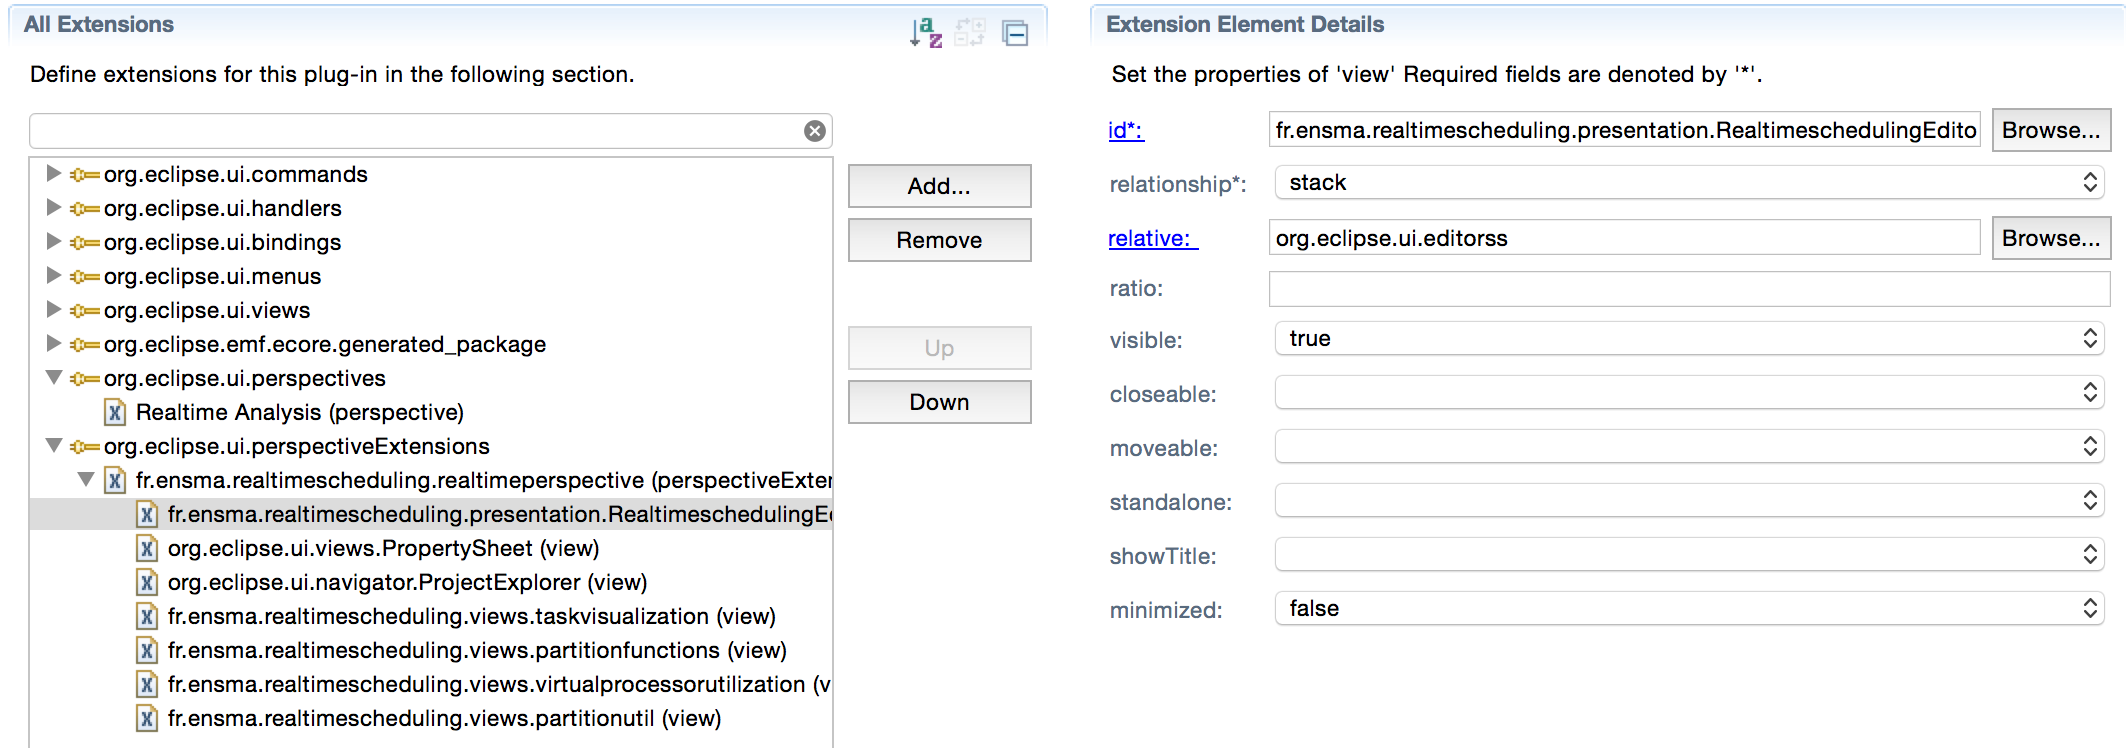
\includegraphics[width=0.5\textwidth]{perspective_extension}
	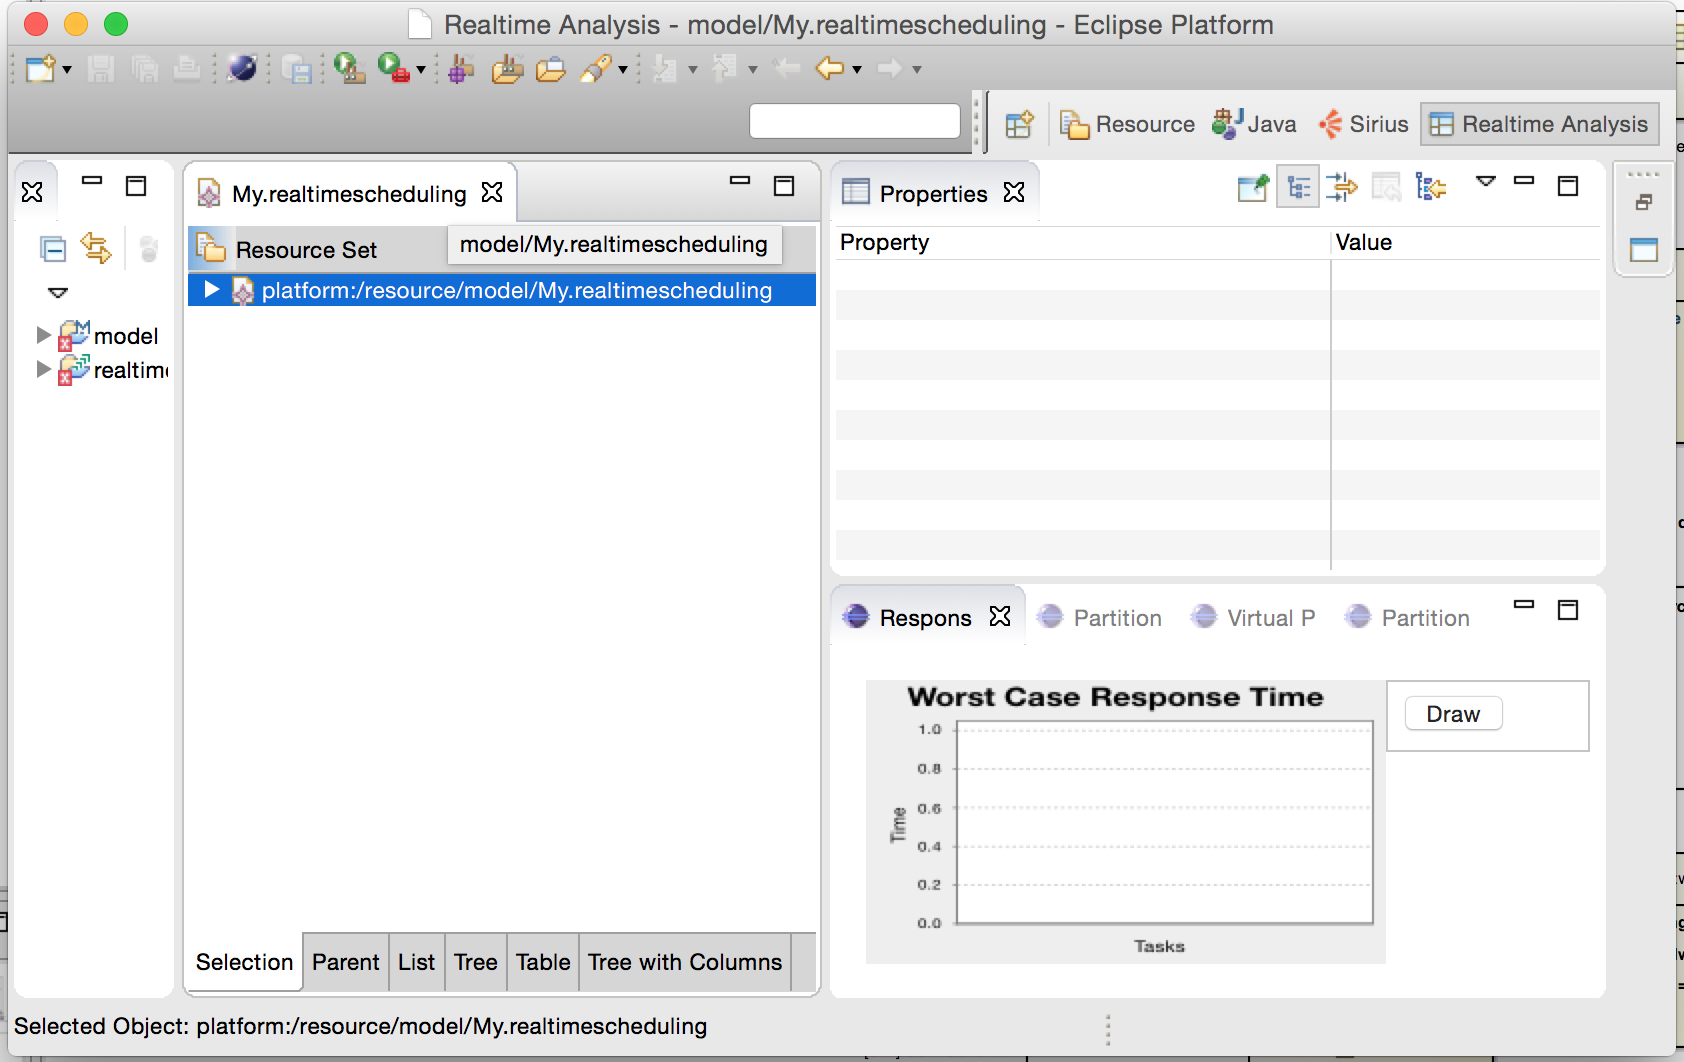
\includegraphics[width=.4\textwidth]{perspective_action}
	\caption{New perspective}
    \end{figure}


\end{description}

